\begin{frame}
\begin{minipage}[t]{.6\textwidth}
\begin{figure}
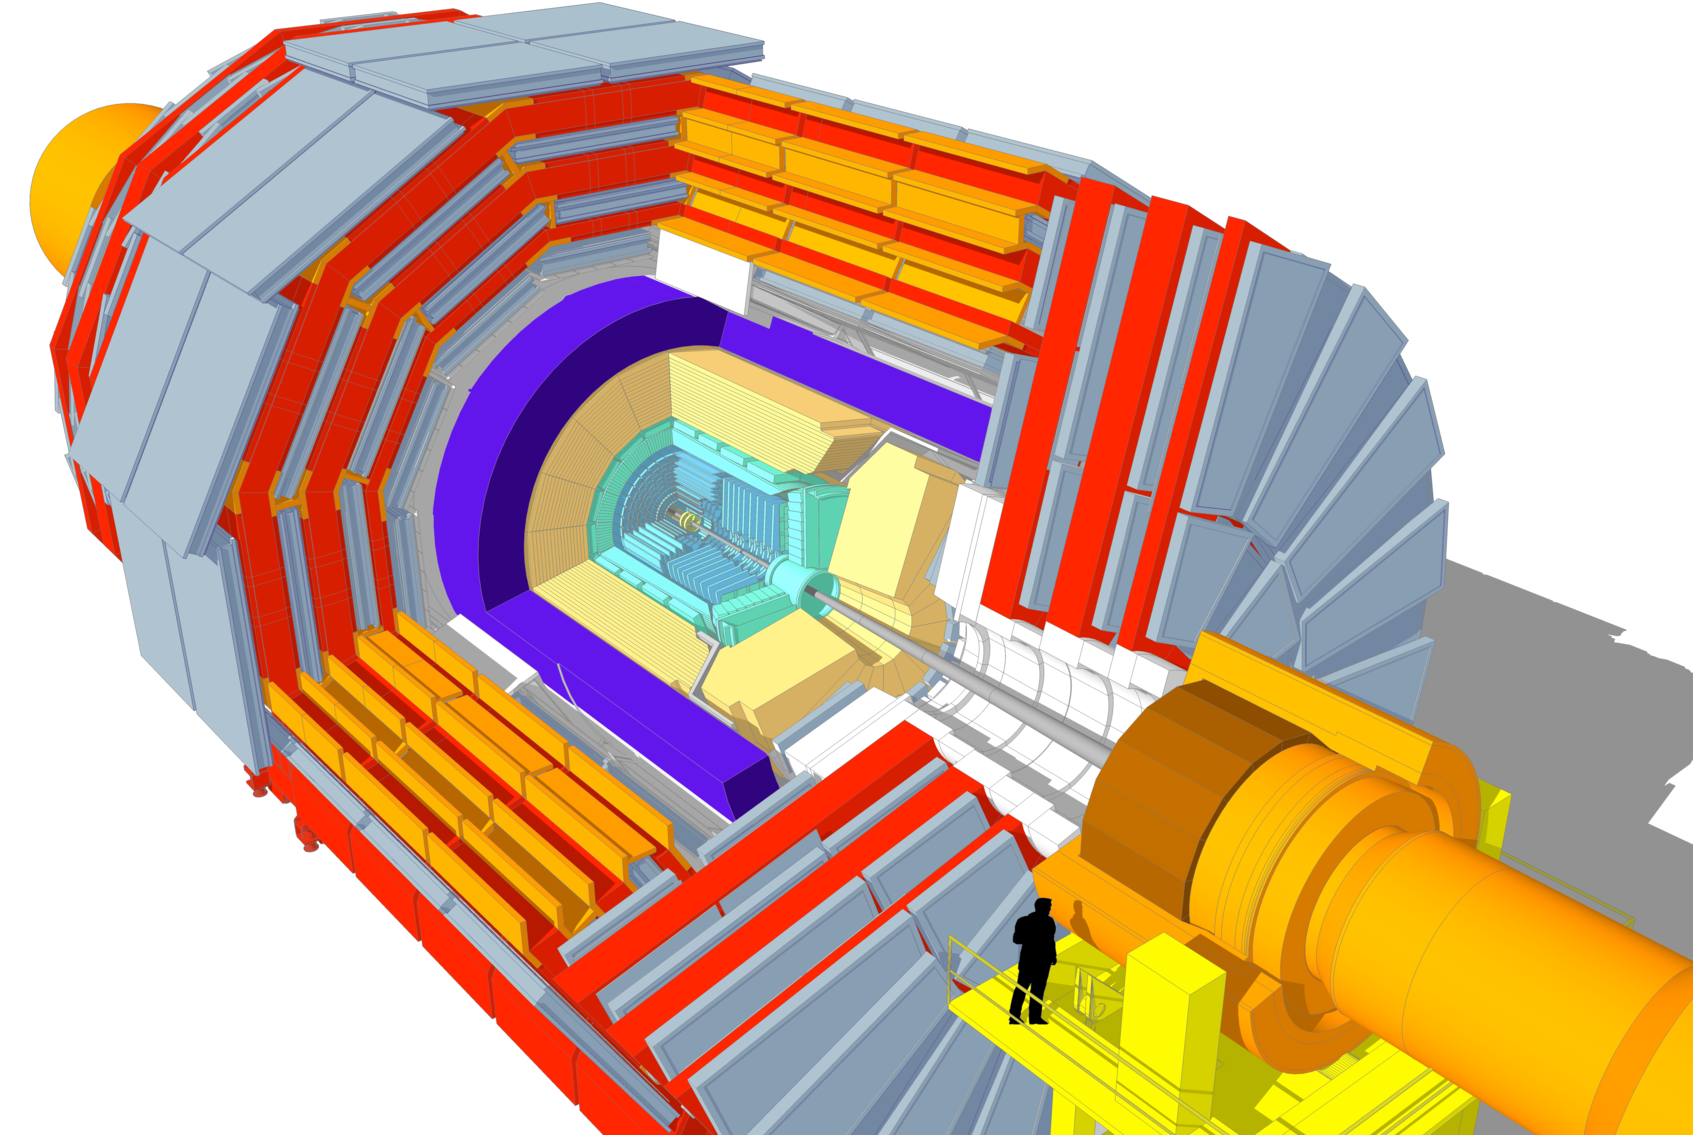
\includegraphics[width=\textwidth,height=\graphh,keepaspectratio]{\PhDthesisdir/plots_and_images/CMS_slices/from_CMS_document_11982-v2/small_cms_full.png}
\end{figure}
\end{minipage}
\hfill\begin{minipage}[t]{.35\textwidth}
\begin{block}{CMS detector}
\begin{itemize}
\item Mass: $\sim\SI{14000}{t}$, $\num{12500}$ only for red part
\item Diameter: \SI{15}{\meter}
\item Length: \SI{28.7}{\meter}
\end{itemize}
\end{block}
\end{minipage}
\end{frame}

\begin{frame}
\addtocounter{framenumber}{-1}
\transdissolve
\begin{minipage}[t]{.6\textwidth}
\begin{figure}
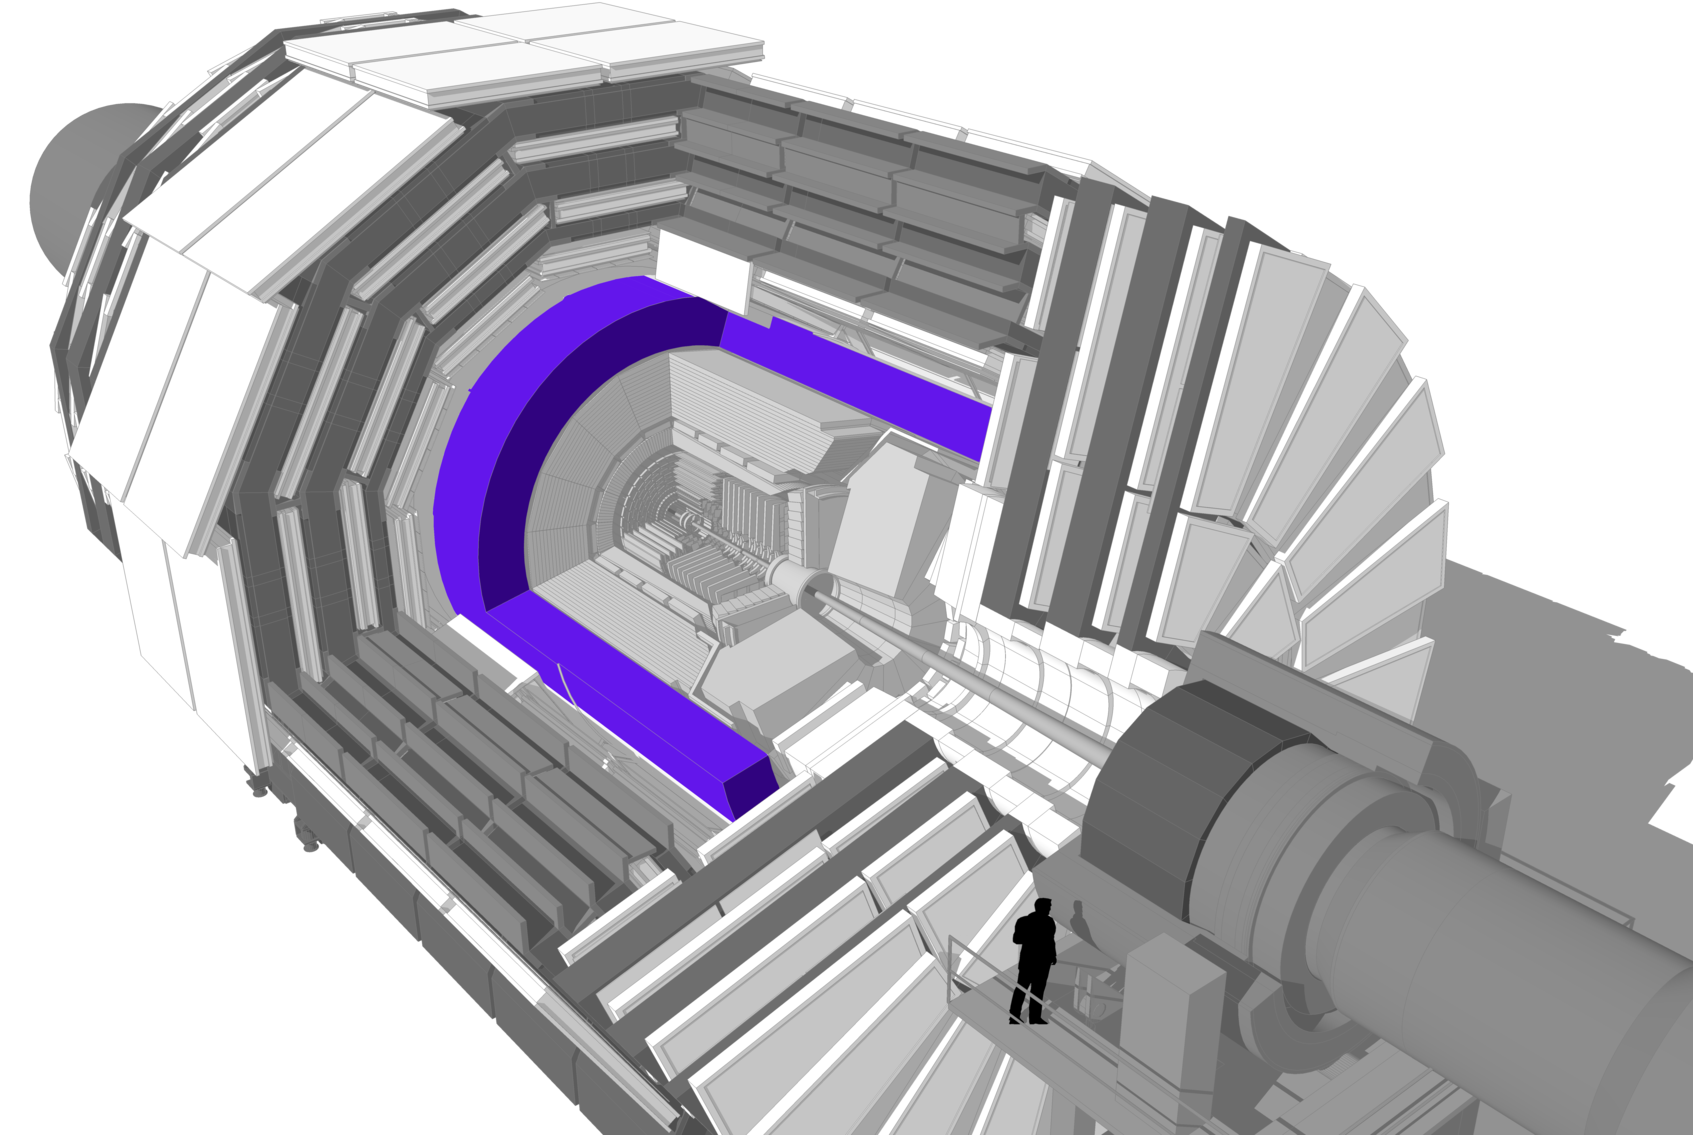
\includegraphics[width=\textwidth,height=\graphh,keepaspectratio]{\PhDthesisdir/plots_and_images/CMS_slices/from_CMS_document_11982-v2/small_cms_solenoid.png}
\end{figure}
\end{minipage}
\hfill\begin{minipage}[t]{.35\textwidth}
\begin{block}{Solenoid}
\begin{itemize}
\item Niobium titanium coil
\item Superconducting
\item $\sim\SI{18000}{\ampere}$
\item \SI{4}{\tesla} in the inner volume
\end{itemize}
\end{block}
\end{minipage}
\end{frame}

\begin{frame}
\addtocounter{framenumber}{-1}
\transdissolve
\begin{minipage}[t]{.6\textwidth}
\begin{figure}
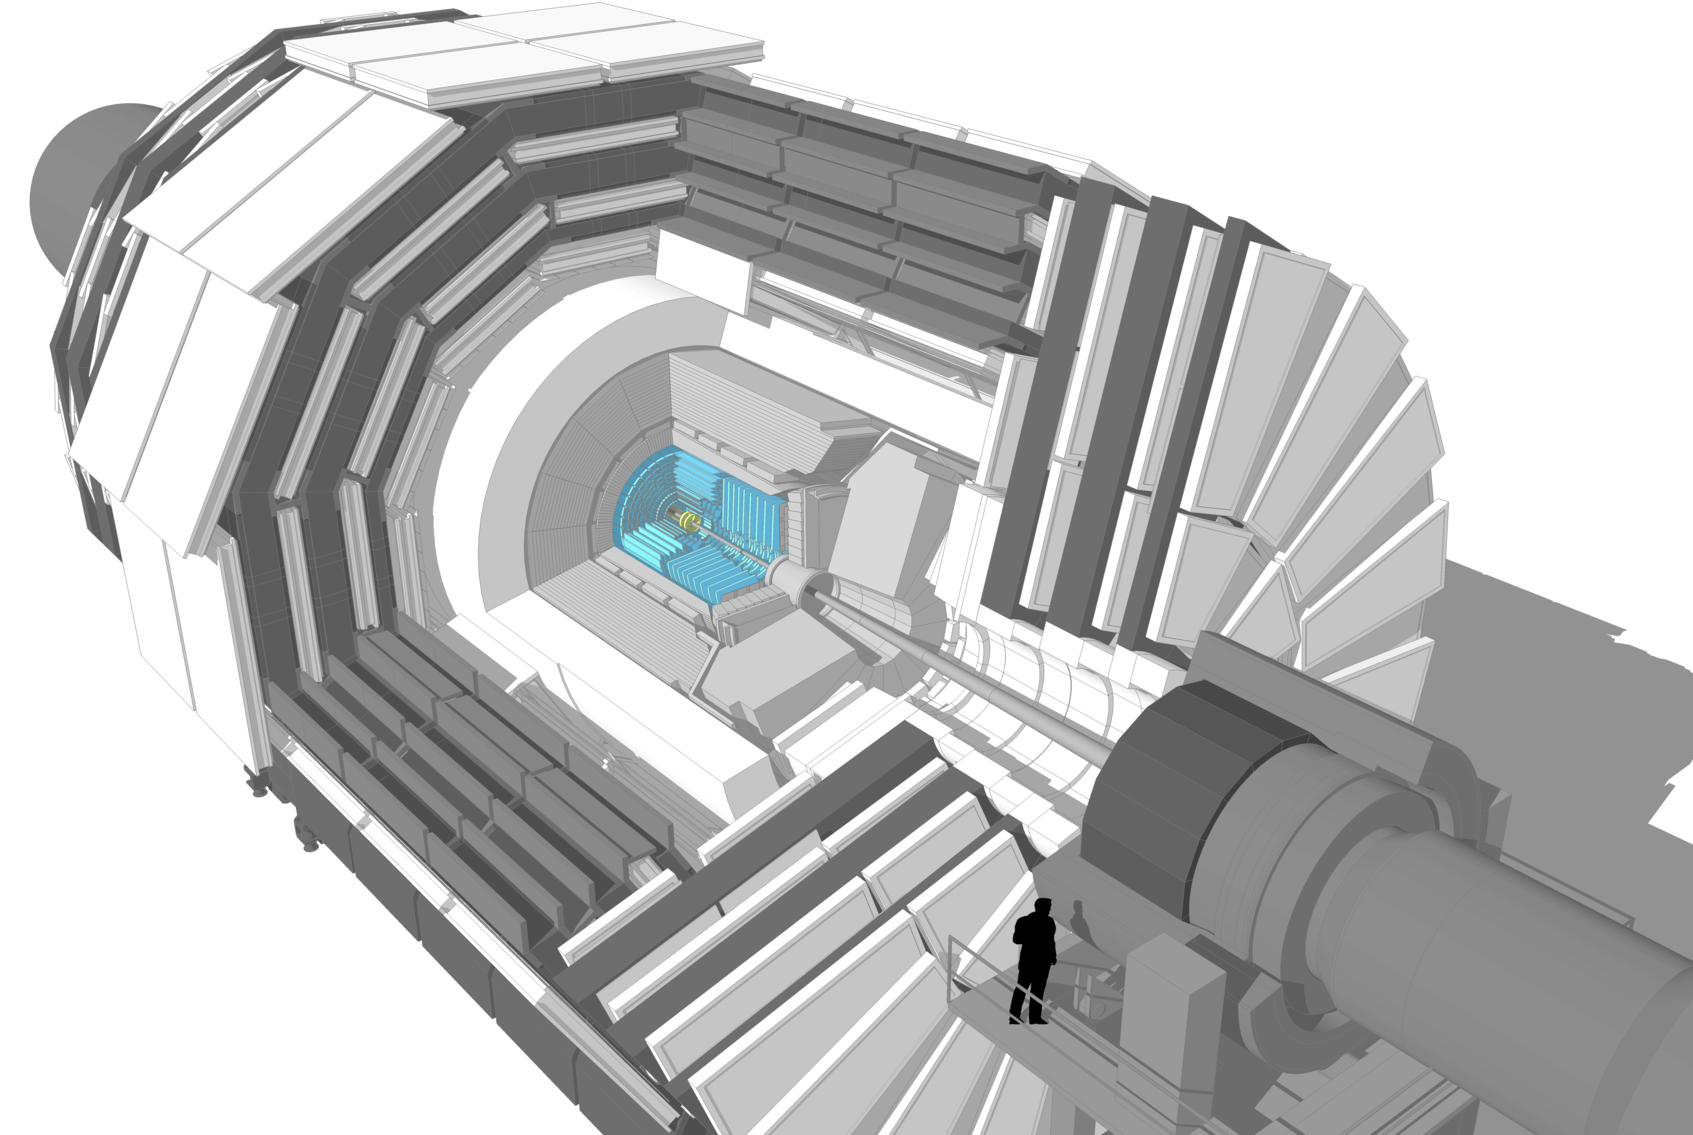
\includegraphics[width=\textwidth,height=\graphh,keepaspectratio]{\PhDthesisdir/plots_and_images/CMS_slices/from_CMS_document_11982-v2/small_cms_tracker.png}
\end{figure}
\end{minipage}
\hfill\begin{minipage}[t]{.35\textwidth}
\begin{block}{Tracker}
\begin{itemize}
\item Inner: pixels ($\num{100}\times\SI{150}{\micro\meter^2}$, $\sim\SI{1.9}{\meter^2}$, $\sim\SI{124}{M}$ channels
\item Outer: microstrips ($\num{80}-\SI{180}{\micro\meter}$) $\sim\SI{200}{\meter^2}$ $\sim\SI{9.6}{M}$ channels
\end{itemize}
\end{block}
\end{minipage}
\end{frame}

\begin{frame}
\addtocounter{framenumber}{-1}
\transdissolve
\begin{minipage}[t]{.6\textwidth}
\begin{figure}
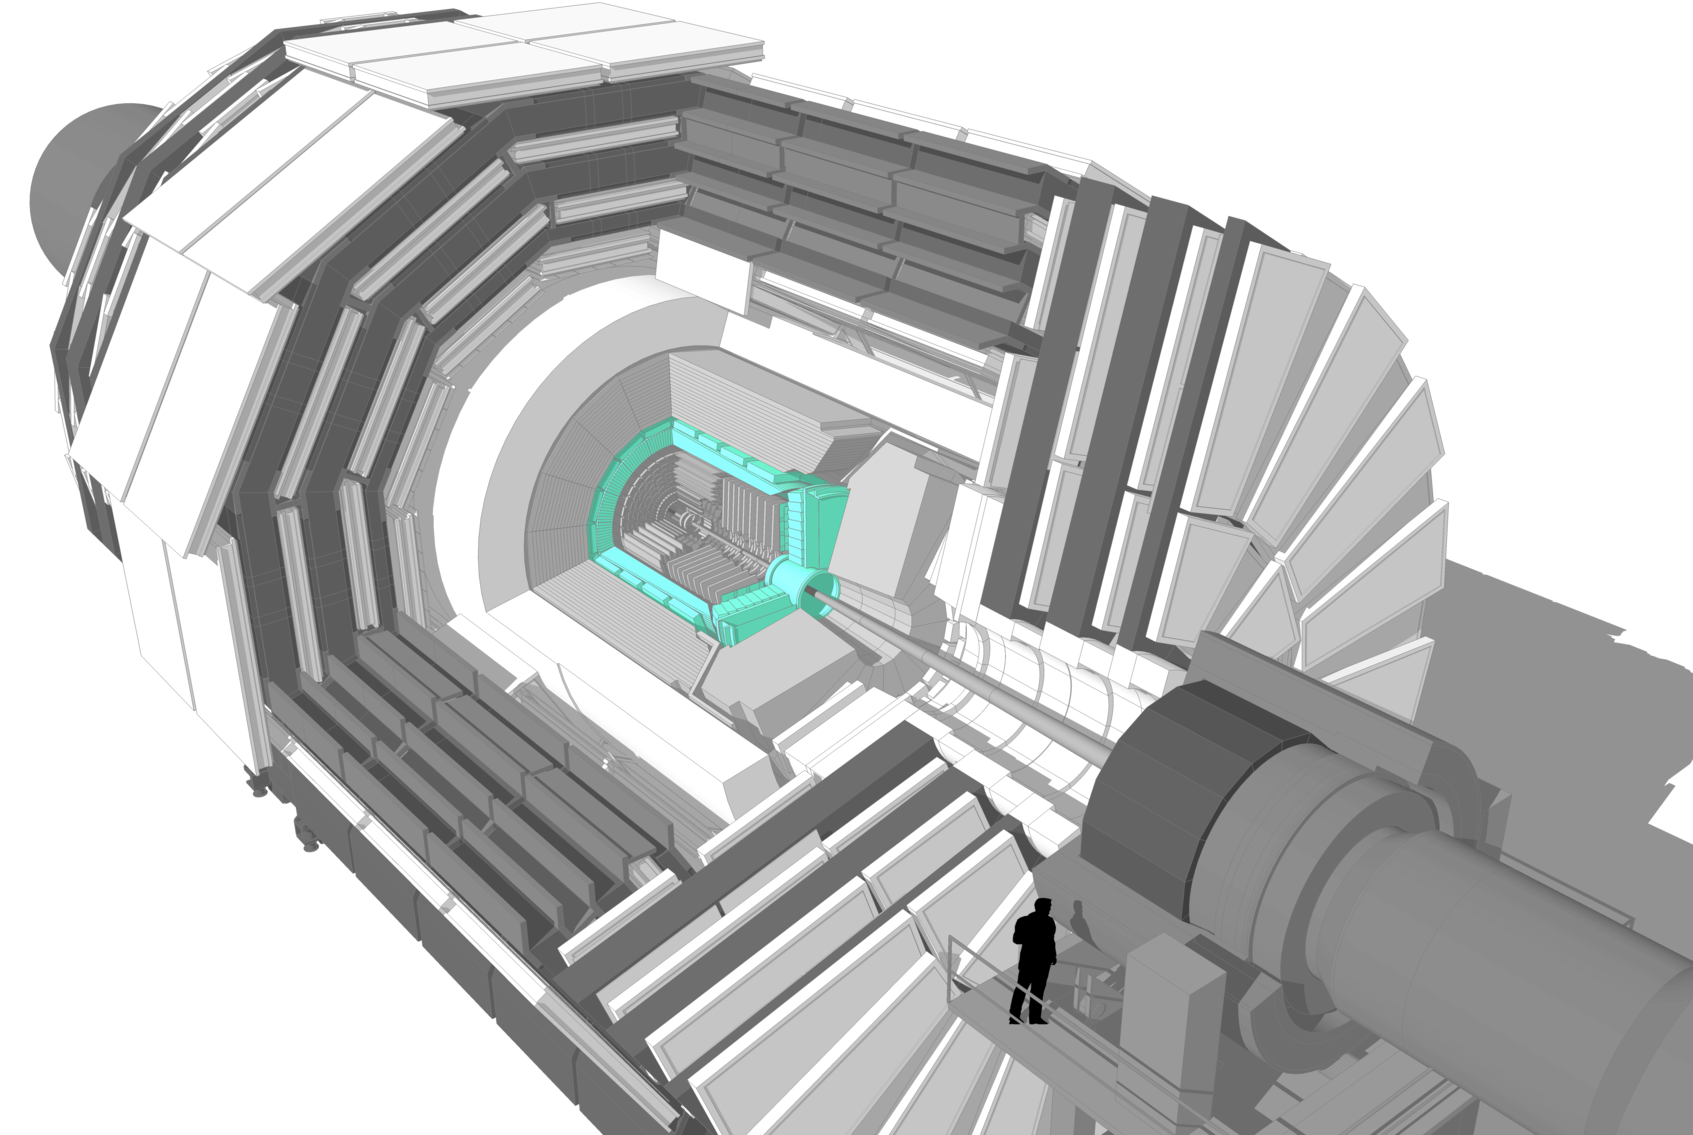
\includegraphics[width=\textwidth,height=\graphh,keepaspectratio]{\PhDthesisdir/plots_and_images/CMS_slices/from_CMS_document_11982-v2/small_cms_ecal.png}
\end{figure}
\end{minipage}
\hfill\begin{minipage}[t]{.35\textwidth}
\begin{block}{Electromagnetic CALorimeter}
\begin{itemize}
\item $\sim\num{76000}$ scintillating \ce{PbWO4} crystals
\end{itemize}
\end{block}
\end{minipage}
\end{frame}

\begin{frame}
\addtocounter{framenumber}{-1}
\transdissolve
\begin{minipage}[t]{.6\textwidth}
\begin{figure}
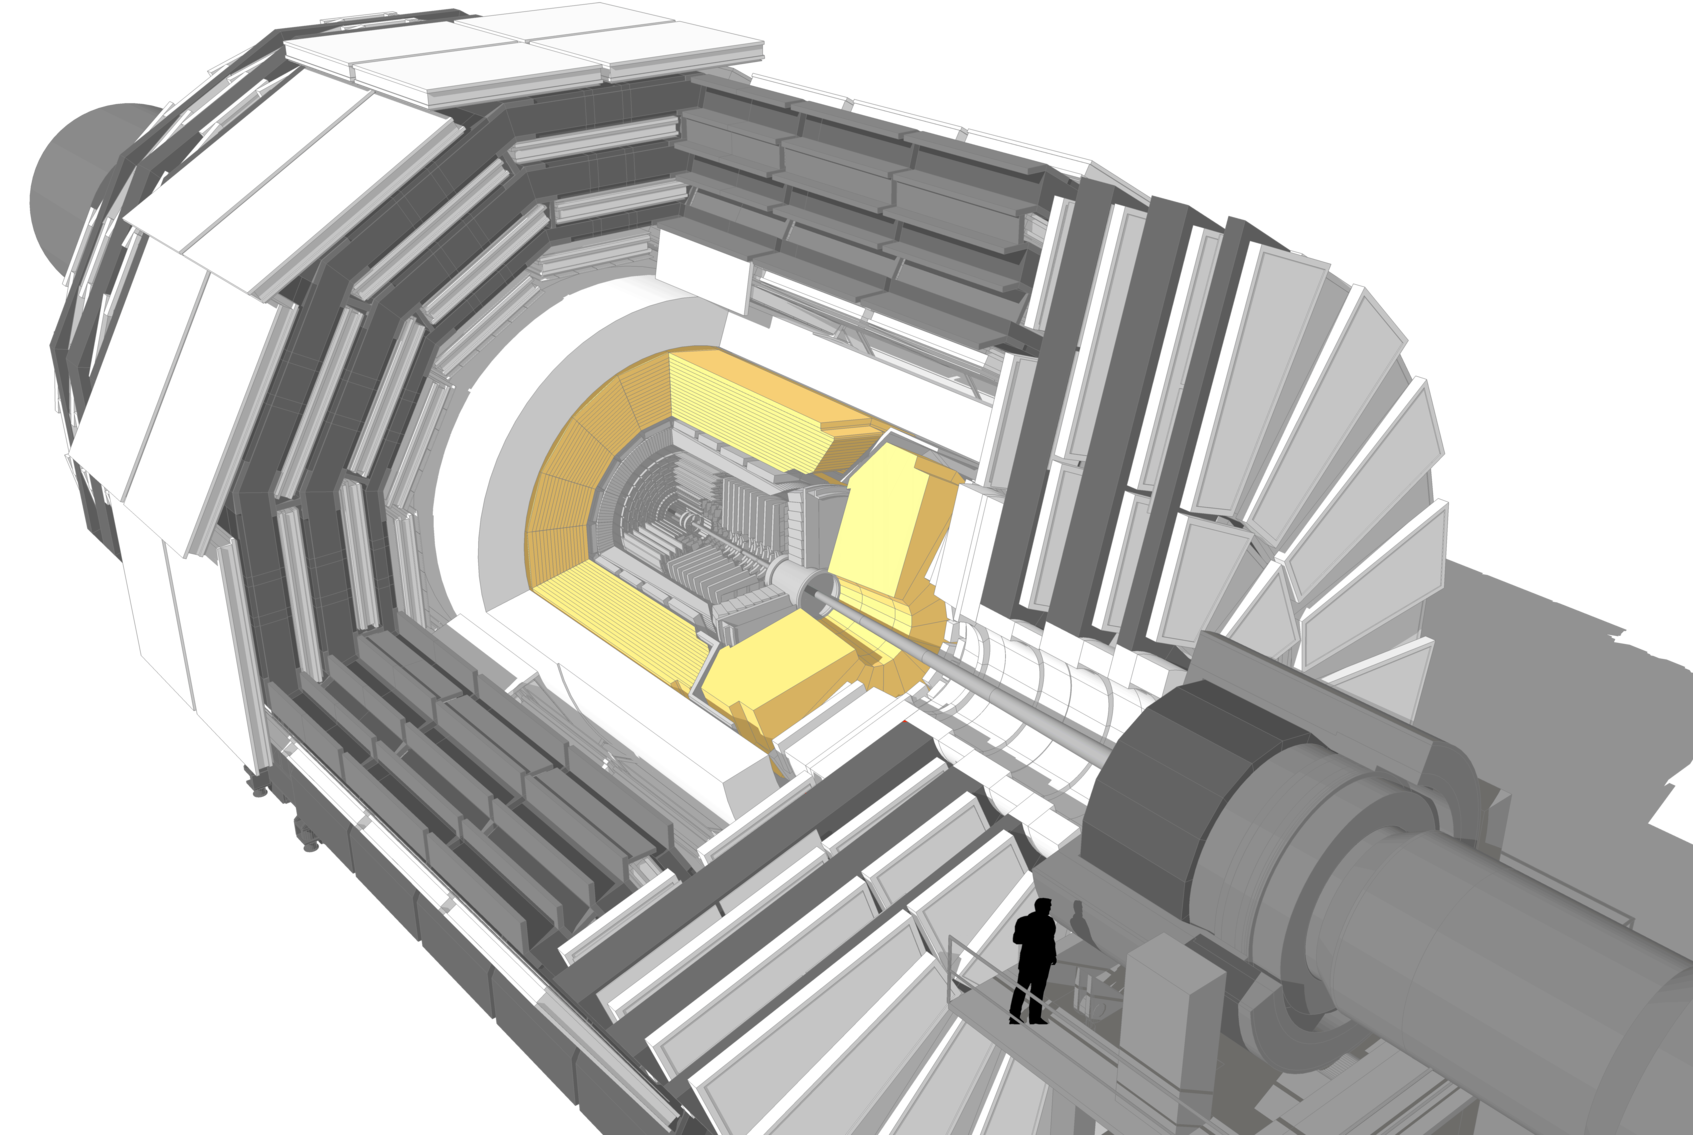
\includegraphics[width=\textwidth,height=\graphh,keepaspectratio]{\PhDthesisdir/plots_and_images/CMS_slices/from_CMS_document_11982-v2/small_cms_hcal.png}
\end{figure}
\end{minipage}
\hfill\begin{minipage}[t]{.35\textwidth}
\begin{block}{Hadronic CALorimeter}
\begin{itemize}
\item brass +, plastic scintillator, $\sim\num{7000}$ channels
\end{itemize}
\end{block}
\end{minipage}
\end{frame}

\begin{frame}
\addtocounter{framenumber}{-1}
\transdissolve
\begin{minipage}[t]{.6\textwidth}
\begin{figure}
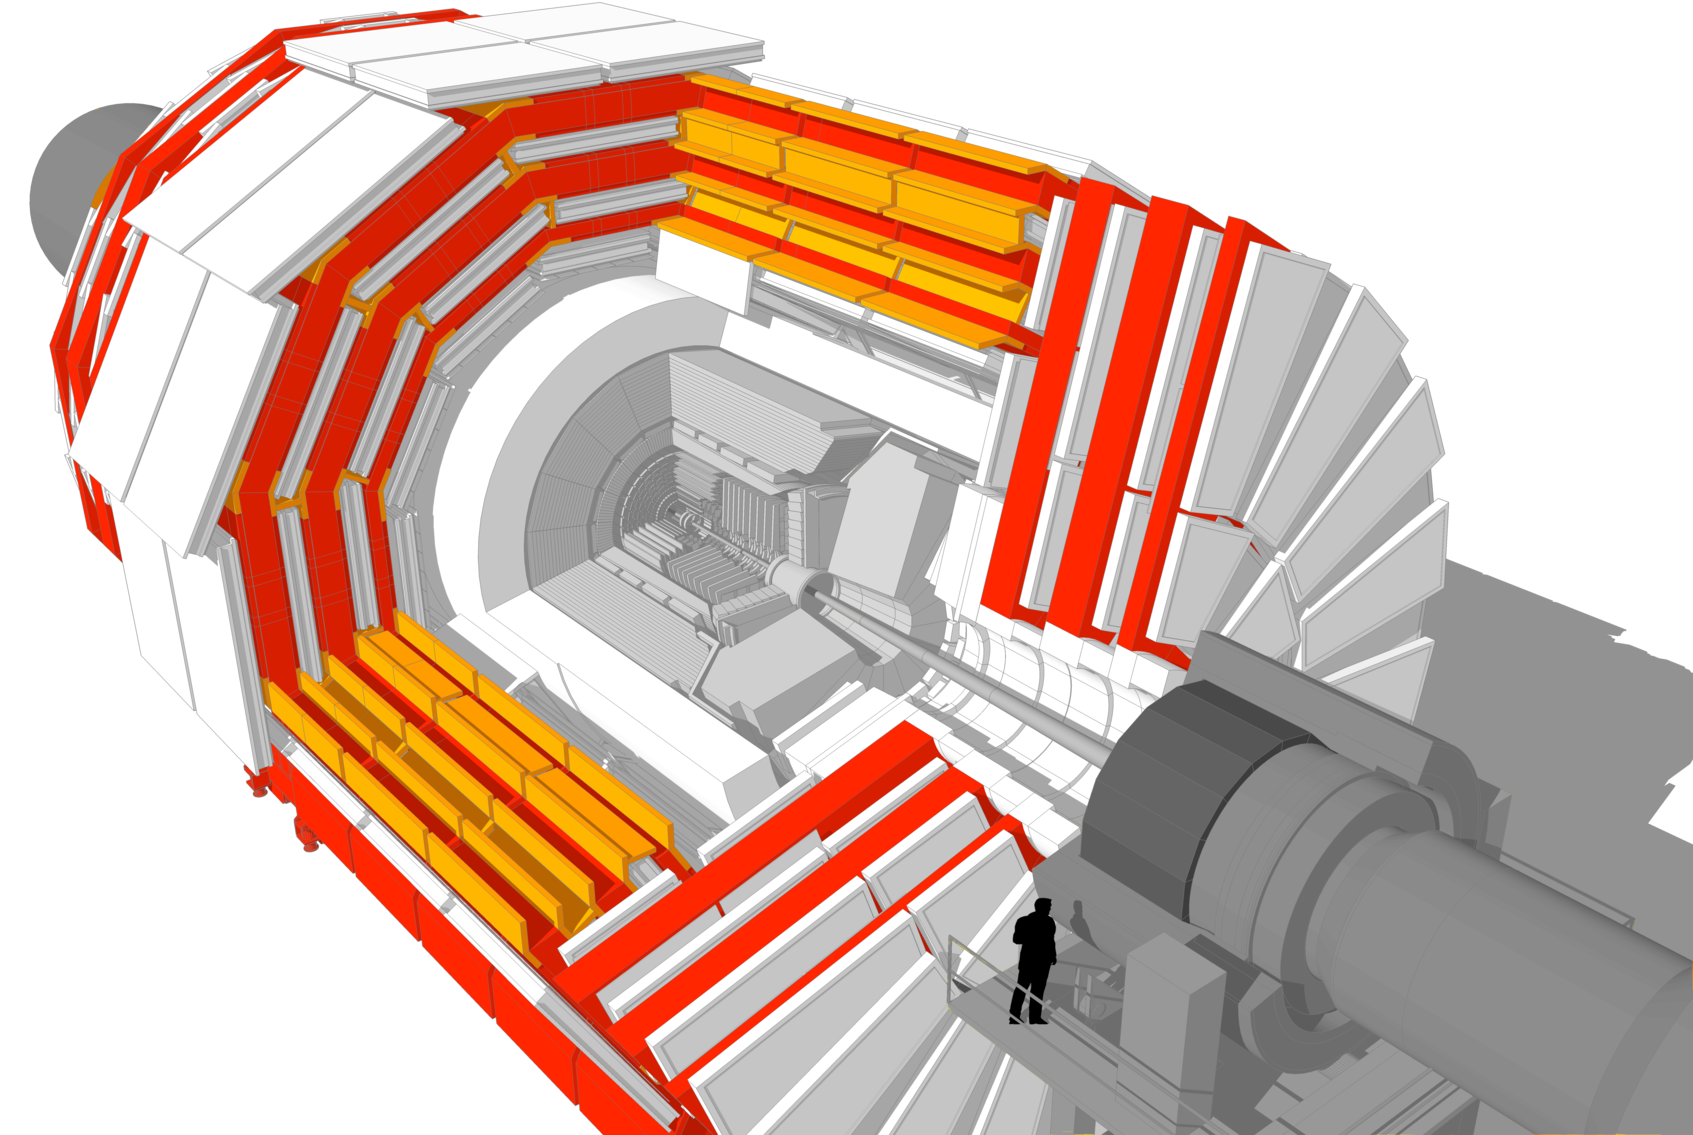
\includegraphics[width=\textwidth,height=\graphh,keepaspectratio]{\PhDthesisdir/plots_and_images/CMS_slices/from_CMS_document_11982-v2/small_cms_muons.png}
\end{figure}
\end{minipage}
\hfill\begin{minipage}[t]{.35\textwidth}
\begin{block}{Muon chambers (white)}
\begin{itemize}
\item Barrel: \num{250} drift tubes, \num{480} resistive plate chambers
\item Endcaps: \num{540} cathode strip, \num{576} resistive plate chambers
\end{itemize}
\end{block}

\begin{block}{Steel return yoke (red)}
\begin{itemize}
\item allows for \SI{2}{\tesla} magnetic field around the solenoid
\end{itemize}
\end{block}
\end{minipage}
\end{frame}

\begin{frame}
\addtocounter{framenumber}{-1}
\transdissolve
\begin{minipage}[t]{.6\textwidth}
\begin{figure}
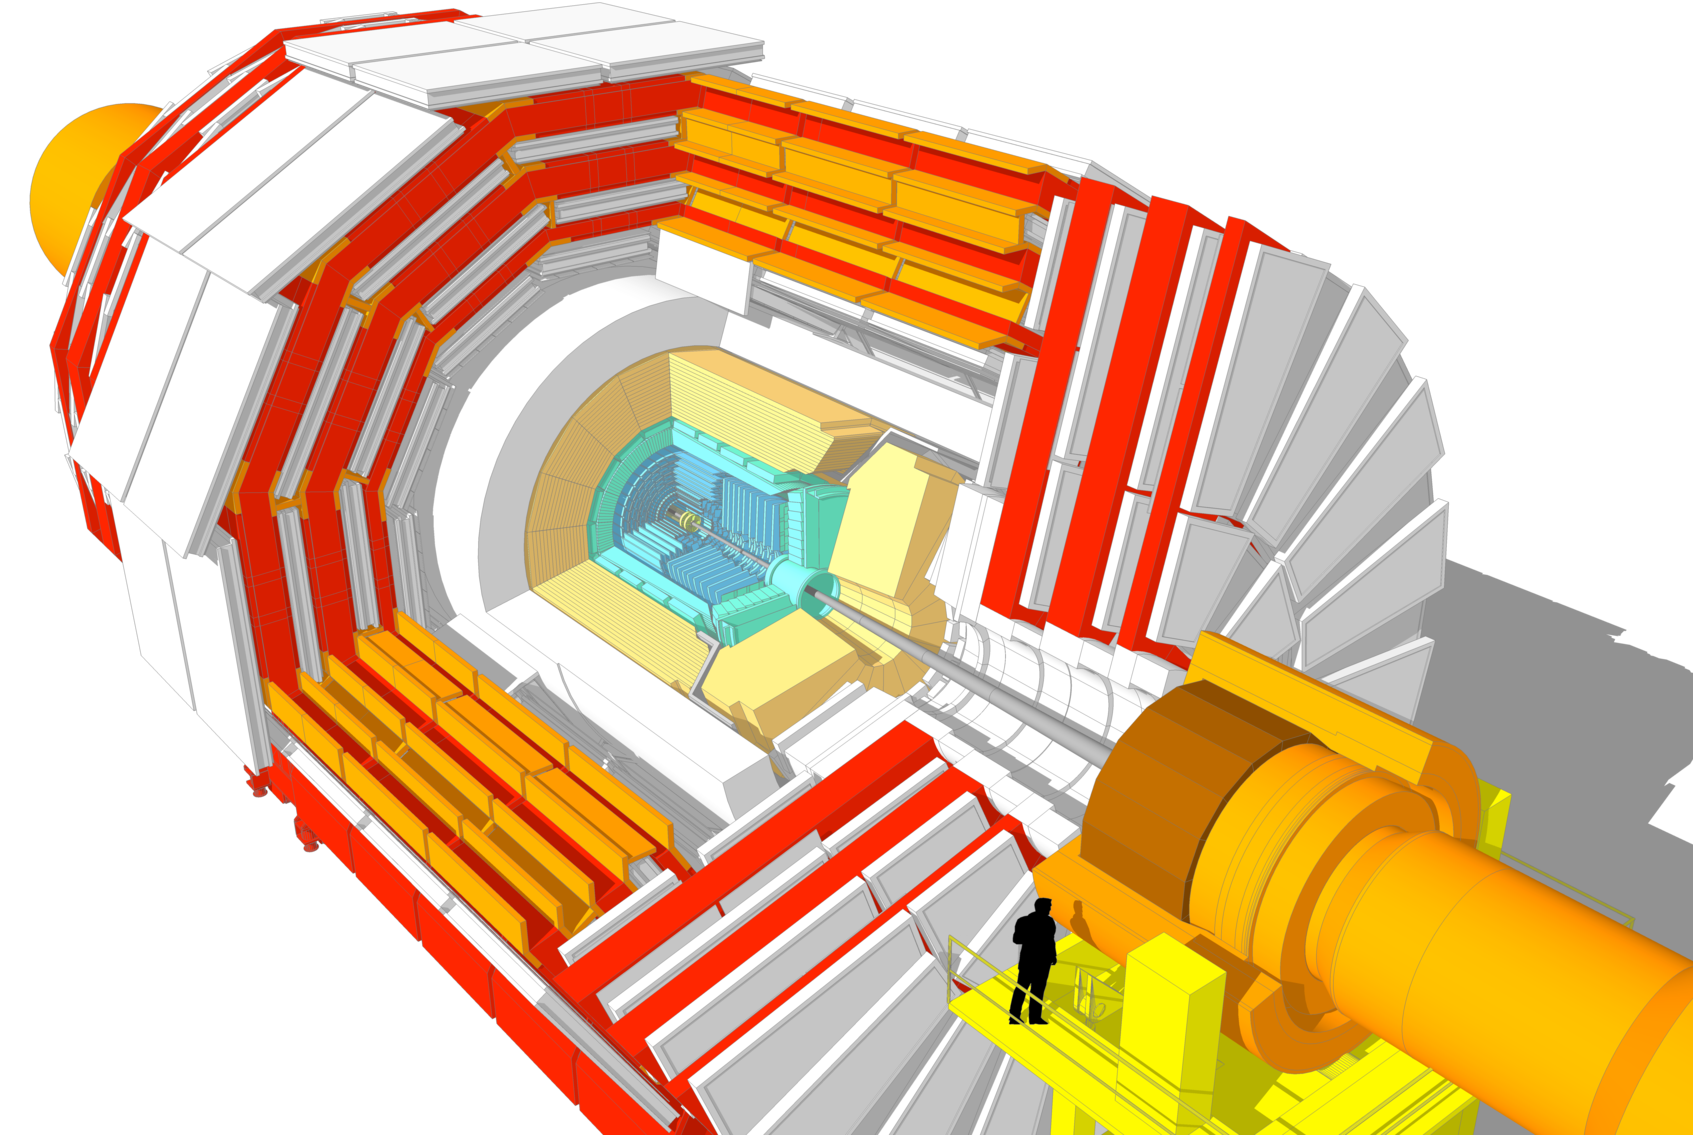
\includegraphics[width=\textwidth,height=\graphh,keepaspectratio]{\PhDthesisdir/plots_and_images/CMS_slices/from_CMS_document_11982-v2/small_cms_full_no_violet_solen.png}
\end{figure}
\end{minipage}
\hfill\begin{minipage}[t]{.35\textwidth}
\begin{block}{}
\begin{itemize}
\item Combine sub-detectors signals to determine particles!
\end{itemize}
\end{block}
\end{minipage}
\end{frame}